\byline{{\textbf{\Large\sffamily January Bonsai Club Meetup:}}\\
{\textbf{\large\sffamily Winter Chills and Spring Preparations}}}{The Newsletter Team}
\noindent
The new year arrived with a sharp reminder of the season as the weather finally took a turn for the worse.
Despite the heavy rain and cold winds that delayed some or kept others at home, we still enjoyed a strong turnout for our first gathering of 2026.

The night featured our \textbf{Tree of the Month} competition, where the theme was \textbf{``Naked Tree, Elm.''}
It was a fantastic opportunity to appreciate the intricate ramification and structural beauty of deciduous species without their summer finery.
Beyond the competition, the room was filled with members working on their own ``gems'' (pun intended!), sharing advices and catching up after the holiday break.

\medskip
While the trees may be dormant, club activity is certainly not.
Our \textbf{Member Education Programme (MEP)} continues to go from strength to strength.
The second session held just a couple of days after our meetup was incredibly popular; you can find a full reportage of the morning's learning on p.~\pageref{2026-01-workshop-mep}.
As a reminder, our next session on \textbf{Saturday, 28th February} will focus on \textbf{repotting and positioning}.
If you haven't secured your spot with \textbf{Tony Ulatowski} or \textbf{Chris Durne} yet, do so quickly!

\medskip
More importantly, the committee is busy completing the line\--up for our upcoming \textbf{Winter Show}.
This year promises to be our best yet, featuring more vendors and new specialty tables, including a dedicated \textbf{Suiseki} display and a standalone \textbf{Mame} exhibit.
The trade and workshop area is already shaping up to be a hub of activity with live demonstrations scheduled throughout the day.
Meanwhile, \textbf{Stefano} has been hard at work finalising the \textbf{2025 Annuary}---a luxurious collection of last year's newsletters that will soon be available for members.

\medskip
We look forward to seeing you all on the \textbf{second Thursday of February} at the Whitton Community Centre for our next meetup.

\medskip
\medskip
\vspace*{-1em}
\begin{window}[2,l,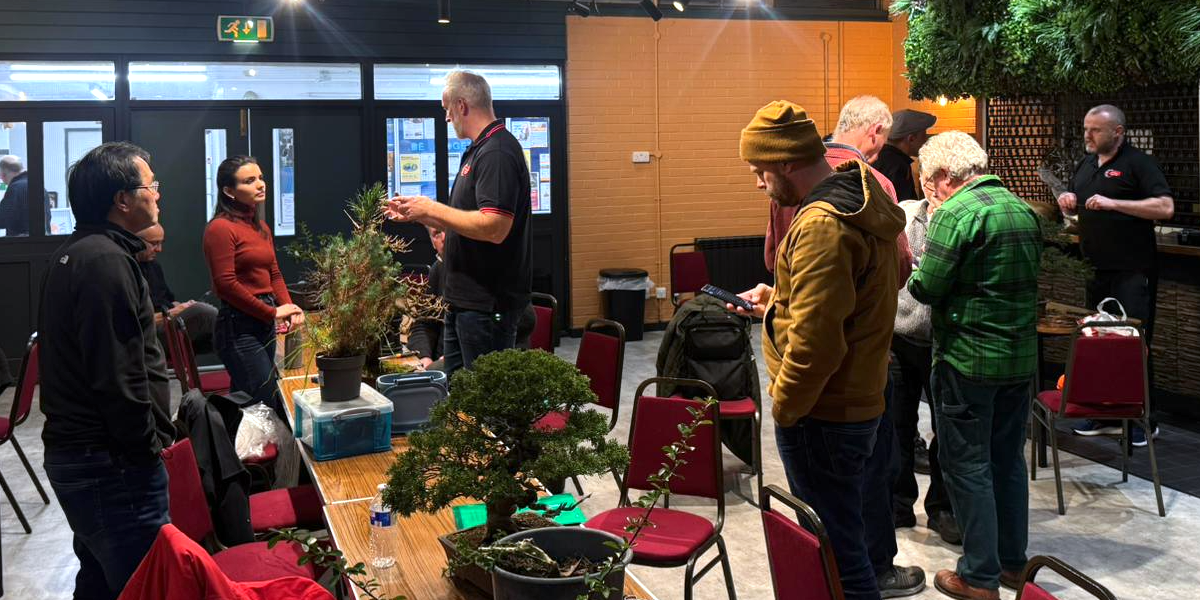
\includegraphics[width=1.0\columnwidth]{2026_01/res/editorial_january},\centerline{\emph{Members braving the winter weather to work on their trees.}}]
\end{window}
\vspace*{-1em}
\closearticle
\clearpage